\documentclass{standalone}
\usepackage{tikz}
\usetikzlibrary{patterns, positioning}
\usepackage[sfdefault]{ClearSans} %% option 'sfdefault' activates Clear Sans as the default text font
\usepackage[T1]{fontenc}

\begin{document}
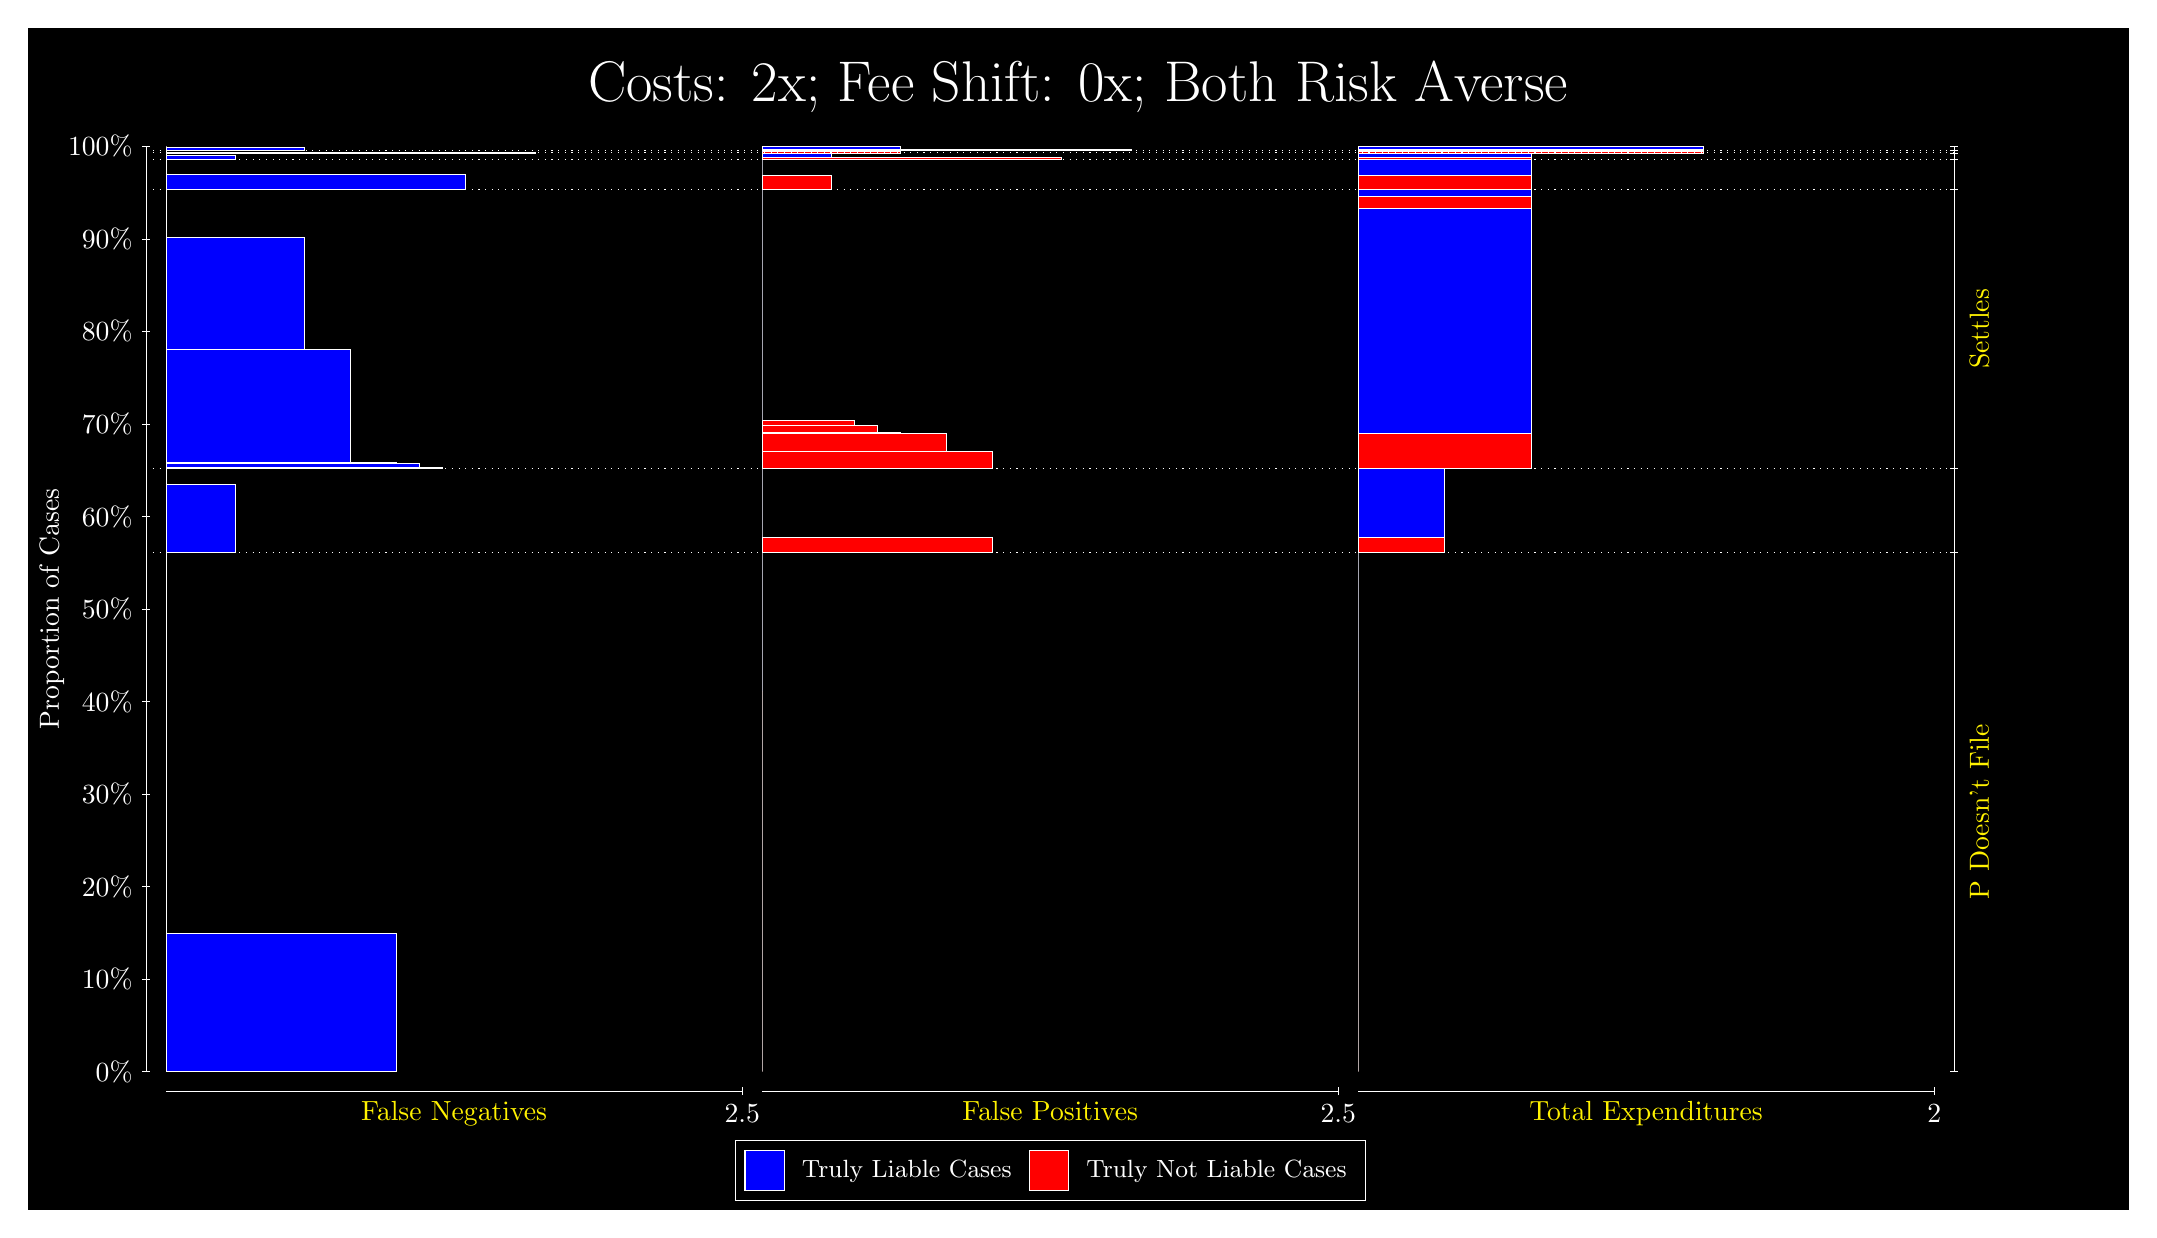
\begin{tikzpicture}
\draw[fill=black] (0,0) rectangle (26.667,15);
\draw[text=white] (0,13.5) rectangle (26.667,15) node[midway] {\huge Costs: 2x; Fee Shift: 0x; Both Risk Averse};
\draw[white, very thin] (1.5,1.75) -- (1.5,13.5);
\node[rotate=90, text=white, anchor=center] at (0.3, 7.625) {Proportion of Cases};
\draw[white, very thin] (1.45,1.75) -- (1.55,1.75);
\node[text=white, anchor=east] at (1.45, 1.75) {0\%};
\draw[white, very thin] (1.45,2.925) -- (1.55,2.925);
\node[text=white, anchor=east] at (1.45, 2.925) {10\%};
\draw[white, very thin] (1.45,4.1) -- (1.55,4.1);
\node[text=white, anchor=east] at (1.45, 4.1) {20\%};
\draw[white, very thin] (1.45,5.275) -- (1.55,5.275);
\node[text=white, anchor=east] at (1.45, 5.275) {30\%};
\draw[white, very thin] (1.45,6.45) -- (1.55,6.45);
\node[text=white, anchor=east] at (1.45, 6.45) {40\%};
\draw[white, very thin] (1.45,7.625) -- (1.55,7.625);
\node[text=white, anchor=east] at (1.45, 7.625) {50\%};
\draw[white, very thin] (1.45,8.8) -- (1.55,8.8);
\node[text=white, anchor=east] at (1.45, 8.8) {60\%};
\draw[white, very thin] (1.45,9.975) -- (1.55,9.975);
\node[text=white, anchor=east] at (1.45, 9.975) {70\%};
\draw[white, very thin] (1.45,11.15) -- (1.55,11.15);
\node[text=white, anchor=east] at (1.45, 11.15) {80\%};
\draw[white, very thin] (1.45,12.325) -- (1.55,12.325);
\node[text=white, anchor=east] at (1.45, 12.325) {90\%};
\draw[white, very thin] (1.45,13.5) -- (1.55,13.5);
\node[text=white, anchor=east] at (1.45, 13.5) {100\%};

\draw[white, very thin] (24.457,1.75) -- (24.457,13.5);
\draw[white, very thin] (24.407,1.75) -- (24.507,1.75);
\node[anchor=west] at (24.407, 1.75) {};
\draw[white, very thin] (24.407,8.341) -- (24.507,8.341);
\node[anchor=west] at (24.407, 8.341) {};
\draw[white, very thin] (24.407,9.4113) -- (24.507,9.4113);
\node[anchor=west] at (24.407, 9.4113) {};
\draw[white, very thin] (24.407,12.95) -- (24.507,12.95);
\node[anchor=west] at (24.407, 12.95) {};
\draw[white, very thin] (24.407,13.335) -- (24.507,13.335);
\node[anchor=west] at (24.407, 13.335) {};
\draw[white, very thin] (24.407,13.416) -- (24.507,13.416);
\node[anchor=west] at (24.407, 13.416) {};
\draw[white, very thin] (24.407,13.445) -- (24.507,13.445);
\node[anchor=west] at (24.407, 13.445) {};
\draw[white, very thin] (24.407,13.5) -- (24.507,13.5);
\node[anchor=west] at (24.407, 13.5) {};

\draw[white, very thin, fill=blue] (1.75,1.75) rectangle (4.6775,3.5104);
\draw[white, very thin, fill=red] (1.75,3.5104) rectangle (1.75,8.341);
\draw[white, very thin, fill=blue] (1.75,8.341) rectangle (2.6283,9.214);
\draw[white, very thin, fill=red] (1.75,9.214) rectangle (1.75,9.4113);
\draw[white, very thin, fill=blue] (1.75,9.4113) rectangle (5.2631,9.4227);
\draw[white, very thin, fill=blue] (1.75,9.4227) rectangle (4.9703,9.4736);
\draw[white, very thin, fill=blue] (1.75,9.4736) rectangle (4.6775,9.4927);
\draw[white, very thin, fill=blue] (1.75,9.4927) rectangle (4.092,10.919);
\draw[white, very thin, fill=blue] (1.75,10.919) rectangle (3.5065,12.346);
\draw[white, very thin, fill=red] (1.75,12.346) rectangle (1.75,12.95);
\draw[white, very thin, fill=blue] (1.75,12.95) rectangle (5.5558,13.15);
\draw[white, very thin, fill=red] (1.75,13.15) rectangle (1.75,13.335);
\draw[white, very thin, fill=blue] (1.75,13.335) rectangle (2.6283,13.388);
\draw[white, very thin, fill=red] (1.75,13.388) rectangle (1.75,13.416);
\draw[white, very thin, fill=blue] (1.75,13.416) rectangle (6.4341,13.429);
\draw[white, very thin, fill=red] (1.75,13.429) rectangle (1.75,13.445);
\draw[white, very thin, fill=blue] (1.75,13.445) rectangle (3.5065,13.487);
\draw[white, very thin, fill=red] (1.75,13.487) rectangle (1.75,13.5);
\draw[white, very thin, fill=red] (9.3189,1.75) rectangle (9.3189,6.5806);
\draw[white, very thin, fill=blue] (9.3189,6.5806) rectangle (9.3189,8.341);
\draw[white, very thin, fill=red] (9.3189,8.341) rectangle (12.246,8.5382);
\draw[white, very thin, fill=blue] (9.3189,8.5382) rectangle (9.3189,9.4113);
\draw[white, very thin, fill=red] (9.3189,9.4113) rectangle (12.246,9.633);
\draw[white, very thin, fill=red] (9.3189,9.633) rectangle (11.661,9.8547);
\draw[white, very thin, fill=red] (9.3189,9.8547) rectangle (11.075,9.8692);
\draw[white, very thin, fill=red] (9.3189,9.8692) rectangle (10.783,9.9612);
\draw[white, very thin, fill=red] (9.3189,9.9612) rectangle (10.49,10.016);
\draw[white, very thin, fill=blue] (9.3189,10.016) rectangle (9.3189,12.95);
\draw[white, very thin, fill=red] (9.3189,12.95) rectangle (10.197,13.136);
\draw[white, very thin, fill=blue] (9.3189,13.136) rectangle (9.3189,13.335);
\draw[white, very thin, fill=red] (9.3189,13.335) rectangle (13.125,13.363);
\draw[white, very thin, fill=blue] (9.3189,13.363) rectangle (10.197,13.416);
\draw[white, very thin, fill=red] (9.3189,13.416) rectangle (11.075,13.432);
\draw[white, very thin, fill=blue] (9.3189,13.432) rectangle (9.3189,13.445);
\draw[white, very thin, fill=red] (9.3189,13.445) rectangle (14.003,13.458);
\draw[white, very thin, fill=blue] (9.3189,13.458) rectangle (11.075,13.5);
\draw[white, very thin, fill=red] (16.888,1.75) rectangle (16.888,6.5806);
\draw[white, very thin, fill=blue] (16.888,6.5806) rectangle (16.888,8.341);
\draw[white, very thin, fill=red] (16.888,8.341) rectangle (17.986,8.5382);
\draw[white, very thin, fill=blue] (16.888,8.5382) rectangle (17.986,9.4113);
\draw[white, very thin, fill=red] (16.888,9.4113) rectangle (19.083,9.8547);
\draw[white, very thin, fill=blue] (16.888,9.8547) rectangle (19.083,12.708);
\draw[white, very thin, fill=red] (16.888,12.708) rectangle (19.083,12.869);
\draw[white, very thin, fill=blue] (16.888,12.869) rectangle (19.083,12.95);
\draw[white, very thin, fill=red] (16.888,12.95) rectangle (19.083,13.136);
\draw[white, very thin, fill=blue] (16.888,13.136) rectangle (19.083,13.335);
\draw[white, very thin, fill=red] (16.888,13.335) rectangle (19.083,13.363);
\draw[white, very thin, fill=blue] (16.888,13.363) rectangle (19.083,13.416);
\draw[white, very thin, fill=red] (16.888,13.416) rectangle (21.279,13.432);
\draw[white, very thin, fill=blue] (16.888,13.432) rectangle (21.279,13.445);
\draw[white, very thin, fill=red] (16.888,13.445) rectangle (21.279,13.458);
\draw[white, very thin, fill=blue] (16.888,13.458) rectangle (21.279,13.5);
\draw[white, dotted] (1.5,8.341) -- (24.457,8.341);
\draw[white, dotted] (1.5,9.4113) -- (24.457,9.4113);
\draw[white, dotted] (1.5,12.95) -- (24.457,12.95);
\draw[white, dotted] (1.5,13.335) -- (24.457,13.335);
\draw[white, dotted] (1.5,13.416) -- (24.457,13.416);
\draw[white, dotted] (1.5,13.445) -- (24.457,13.445);
\draw[white, very thin] (1.75,1.5) -- (9.0689,1.5);
\node[text=yellow, anchor=north] at (5.4094, 1.5) {False Negatives};
\draw[white, very thin] (9.0689,1.45) -- (9.0689,1.55);
\node[text=white, anchor=north] at (9.0689, 1.45) {2.5};

\draw[white, very thin] (9.3189,1.5) -- (16.638,1.5);
\node[text=yellow, anchor=north] at (12.978, 1.5) {False Positives};
\draw[white, very thin] (16.638,1.45) -- (16.638,1.55);
\node[text=white, anchor=north] at (16.638, 1.45) {2.5};

\draw[white, very thin] (16.888,1.5) -- (24.207,1.5);
\node[text=yellow, anchor=north] at (20.547, 1.5) {Total Expenditures};
\draw[white, very thin] (24.207,1.45) -- (24.207,1.55);
\node[text=white, anchor=north] at (24.207, 1.45) {2};

\node[text=yellow, centered, rotate=90] at (24.777, 5.0455) {P Doesn't File};

\node[text=yellow, centered, rotate=90] at (24.777, 11.181) {Settles};





\draw (12.978300999999998,1.5) node[draw=none] (baseCoordinate) {};
\begin{scope}[align=center]
        \matrix[scale=0.5, draw=white, below=0.5cm of baseCoordinate, nodes={draw}, column sep=0.1cm]{
            \node[rectangle, draw, minimum width=0.5cm, minimum height=0.5cm, fill=blue] {}; &
            \node[draw=none, font=\small, text=white] (B) {Truly Liable Cases}; &
            \node[rectangle, draw, minimum width=0.5cm, minimum height=0.5cm, fill=red] {}; &
            \node[draw=none, font=\small, text=white] (B) {Truly Not Liable Cases}; \\
            };
\end{scope}

\end{tikzpicture}
\end{document}